% ----- formatovani dokumentu -----------------------------------------------
\documentclass[12pt,a4paper,titlepage,final]{report}
\usepackage[utf8]{inputenc}
\usepackage[T1, IL2]{fontenc}
\usepackage{graphicx}
\usepackage{epstopdf}
\usepackage[margin=2cm]{caption}
\usepackage[top=3cm, left=2cm, right=2cm, text={17cm, 24cm}, ignorefoot]{geometry}
\usepackage{color}

% ------ commands -----------------------

\newcommand{\abstractpage}{
\cleardoublepage
\noindent
\chapter*{Abstrakt}
}

% ---------------------------------------

\usepackage{url}
\usepackage{setspace}
\singlespacing
\usepackage[square, numbers]{natbib} 
\pagestyle{plain}
\pagenumbering{arabic}
\setcounter{page}{1}

\setlength{\parindent}{1cm}	
\usepackage{natbib}


% ----- vyberte jazyk -------------------------------------------------------
\usepackage[english,czech]{babel}
%\usepackage[english]{babel}

% ----- dopiste titulky -----------------------------------------------------
\newcommand\Course{Fyzikální optika}
\newcommand\WorkTitle{Digitální fotografie - snímače, RAW a zpracování obrazu}
\newcommand\AuthorA{Pavel Macenauer}
\newcommand\AuthorAEmail{pavel.macenauer@fotoaparat.cz}
\newcommand\Faculty{Fakulta Informačních Technologií}
\newcommand\School{Vysoké Učení Technické v Brně}

\usepackage[
pdftitle={\WorkTitle},
pdfauthor={\AuthorA},
bookmarks=true,
colorlinks=true,
breaklinks=true,
urlcolor=blue,
citecolor=blue,
linkcolor=blue,
unicode=true,
]
{hyperref}


% ----- titulni strana ------------------------------------------------------

\begin{document}
	\begin{titlepage}
	\begin{center}
		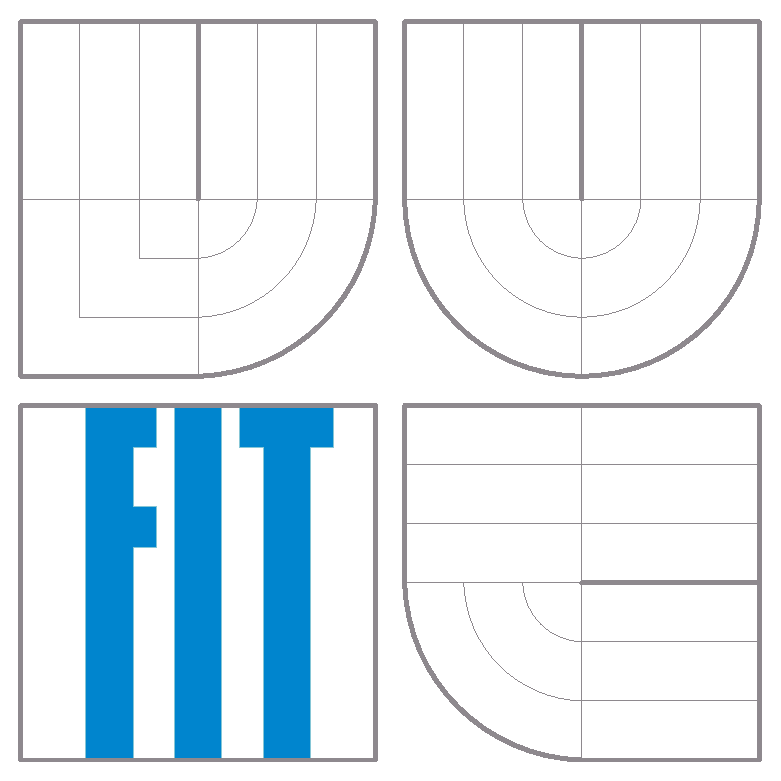
\includegraphics[height=5cm]{images/logo.eps}
	\end{center}
	\vfill
	\begin{center}
		\begin{Large}
			\Course\\
		\end{Large}
		\bigskip
		\begin{Huge}
			\WorkTitle\\
		\end{Huge}
	\end{center}
	\vfill
	\begin{center}
		\begin{large}
			\today
		\end{large}
	\end{center}
	\vfill
	\begin{flushleft}
		\begin{large}
			\begin{tabular}{lll}
				Autor: & \AuthorA, & \url{\AuthorAEmail} \\
		
				& & \\
				& \Faculty \\
				& \School \\
			\end{tabular}
		\end{large}
	\end{flushleft}
\end{titlepage}		

% ----- abstrakt --------------------------------------------------------------
	
\abstractpage

V moderních digitálních fotoaparátech se používají dva typy obrazových snímačů - CCD a CMOS. Každý má své výhody i nevýhody. CMOS snímače dnes nabývají na popularitě především pro své nižší výrobní náklady a větší multimediální využití. CCD jsou oproti tomu stále využívány, je-li třeba kvalitnějšího výstupu. Výstup z těchto snímačů je v podobě RAW. Společnost Adobe Systems Inc. se pokusila vytvořit standard pro RAW výstup, který sice nebyl převzat výrobci digitálních fotoaparátu, ale vzhledem k veřejně dostupné dokumentaci, lze tento formát zpracovat do podoby obrazu a ukázat tak, co vše je třeba provést při zpracování dat z obrazového snímače do zobrazitelné podoby.

\paragraph{Klíčová slova} obrazové snímače - CMOS - CCD - RAW - demozaikování - DNG

	
% ----- obsah --------------------------------------------------------------
	
\tableofcontents

\listoffigures

% ----- obsah -------------------------------------------------------------
\newpage
\chapter{Snímače}

Snímače nebo taktéž obrazové senzory jsou zařízení, která převádějí obraz viditelný např. lidským okem na elektrický signál. Najdeme je ve velkém množství zařízení - od videokamer, přes mobilní telefony po digitální fotoaparáty.

\begin{figure}[ht]
\begin{center}
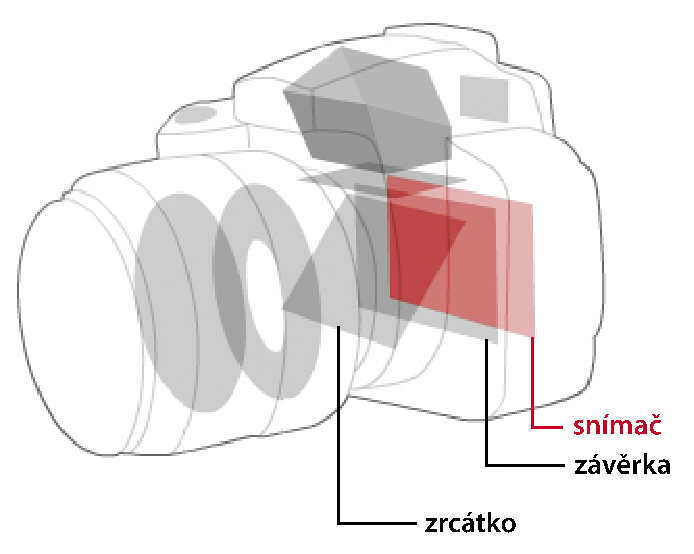
\includegraphics[width=8cm]{images/sensor.pdf}
\caption{Snímač v digitální zrcadlovce}
\label{fig:snimac}
\end{center}
\end{figure}

Jsou složeny z velkého množství obrazových bodů (pixelů). Počet pixelů se uvádí v Mpx (\textbf{megapixelech} \footnote{Větší počet megapixelů neznamená nutně kvalitnější obraz. Naopak kvalita obrazu je závislá více na optické kvalitě objektivu. Pro představu - na výsledném obrazu už je jedno, zda-li máme rozmazanou skrvnu přes 9 nebo přes 4 pixely, důležitější je, aby se nejednalo o rozmazanou skrvnu, ale o ostrý objekt.}), kde každý pixel odpovídá pixelu na výsledném obrazu. U většiny běžných moderních digitálních fotoaparátů se dnes tato hodnota pohybuje mezi 10-ti Mpx u amatérských kompaktních fotoaparátů po 40 u profesionálních digitálních zrcadlovek (\textbf{DSLR} \footnote{Digital Single-Lens Reflex Camera - Digitální zrcadlovka}).

Počet pixelů však neudává velikost nebo poměr šířky a výšky snímače. Poměr stran snímače záleží na výrobci, nejběžnější je 3:2 nebo 4:3 a má vliv pouze na výsledný poměr stran obrazu. Zajímavější je samotná velikost snímače, která má vliv i na kvalitu obrazu. 

\section{Velikost snímače}
Opět existují senzory všech možných velikostí, které se liší na základě toho jak je daná společnost navrhla. Za 2 specifické rozměry u DSLR považujeme \textbf{full-frame} a \textbf{APS-C}.

\subsection{Full-frame}
Full-frame je velikost senzoru stejná jako velikost obrazu u klasický 35mm filmů (tj. 36x24mm). Výhodou je nižší šum za špatných světelných podmínek a větší dynamický rozsah. Nevýhodou však až 20-ti násobné náklady na výrobu a tím pádem i cena fotoaparátu.

\subsection{APS-C} Celým názvem Advanced Photo System type-C je velikost snímače nacházející se u většiny běžných DSLR. Standardizovaně se jedná o 25,1x16,7mm, nicméně dnes jsou tak označovány všechny podobné snímače i mírně odlišných rozměrů. Další nevýhodou, ale i výhodou těchto snímačů oproti svým větším kolegům je, že i když ohnisková vzdálenost zůstává stejná, je plocha snímače menší. Obraz promítaný na snímač je tak užší, což ve výsledku zvětšuje obraz. Resp. výsledný obraz se chová, jako kdyby byl fotografován objektivem s větší ohniskovou vzdáleností. Nelze tak dosáhnout zdaleka takové šířky úhlu záběru, na druhou stranu nám fotoaparát nabízí větší zvětšení, což je vhodné především pro fotografii zvěře nebo sportu.

\subsection{Crop factor}

Nazývá se tak poměr mezi velikostí senzoru a velikostí full-frame senzoru. Lze spočítat pomocí následujícího vzorečku, kde $diag$ je úhlopříčka senzoru:

$$CF = diag_{35mm} / diag_{sensor}$$

Výsledný obraz má tak stejné zvětšení jako kdyby byl fotografován objektivem s ohniskovou vzdáleností:

$$f_{aps-c} = CF * f_{0}$$

Pro většinu výrobců (Nikon, Pentax, Samsung, Sony, Fujifilm, Sigma atd.) je specifické $CF = 1,5$. Vyjímkou jsou fotoaparáty Canon, kde $CF = 1,6$.

\section{Technologie}

Existují dvě základní a velmi odlišná provedení senzorů - CMOS a CCD. Většina výrobců pak má vlastní postupy, kterými pouze dvě výše zmíněné 
technologie zdokonaluje.

\begin{figure}[ht]
\begin{center}
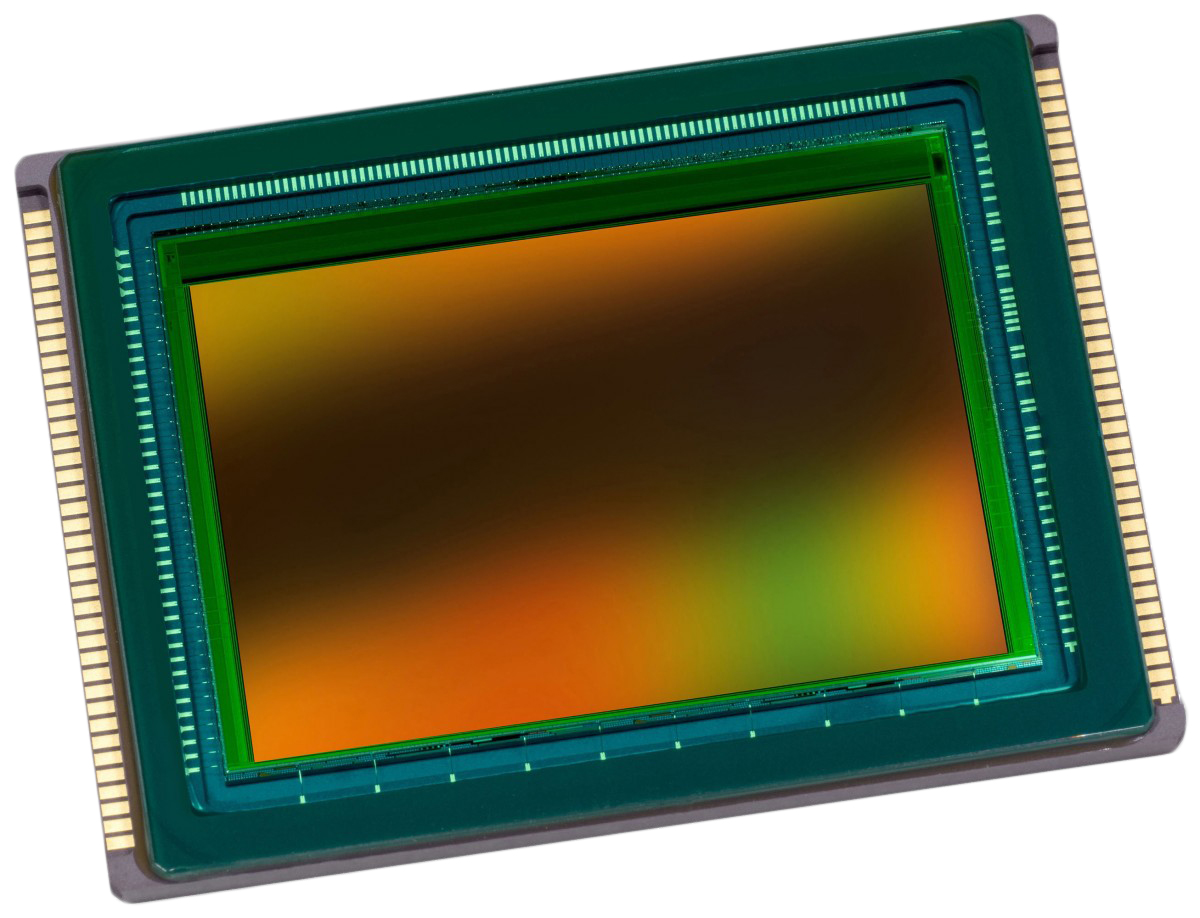
\includegraphics[width=8cm]{images/cmos-real.jpg}
\caption{CMOS snímač}
\label{fig:cmos-real}
\end{center}
\end{figure}

\subsection{CCD}\label{sebsec:ccd}

CCD\footnote{Charge-couple device, v překladu zařízení s vázanými náboji} vynalezl Willard Boyle a George E. Smith v Bellových laboratořích v roce 1969. Roku 2009 za tento vynález obdrželi Nobelovu cenu za fyziku.

Úsměvné může být, že samotní vědci popisují vývoj asi tak, že si během hodiny něco načrtli, a pak to šli jen tak do laboratoře zrealizovat.

V jednoduchosti lze princip jak CCD funguje popsat v následujících krocích: 

		\begin{enumerate}		
			\item otevře se závěrka a na \textbf{polovodič} dopadají fotony generující elektrony/díry
			\item závěrka se uzavře, generace elektronů/děr končí
			\item postupně se nabíjejí elektrody z jedné strany na druhou, ke kterým se posouvají elektrony
			\item zesilovač na konci "polovodičového kanálu" zesílí proud na zpracovatelnou napěťovou úroveň
		\end{enumerate}	
		
		\begin{figure}[ht]
\begin{center}
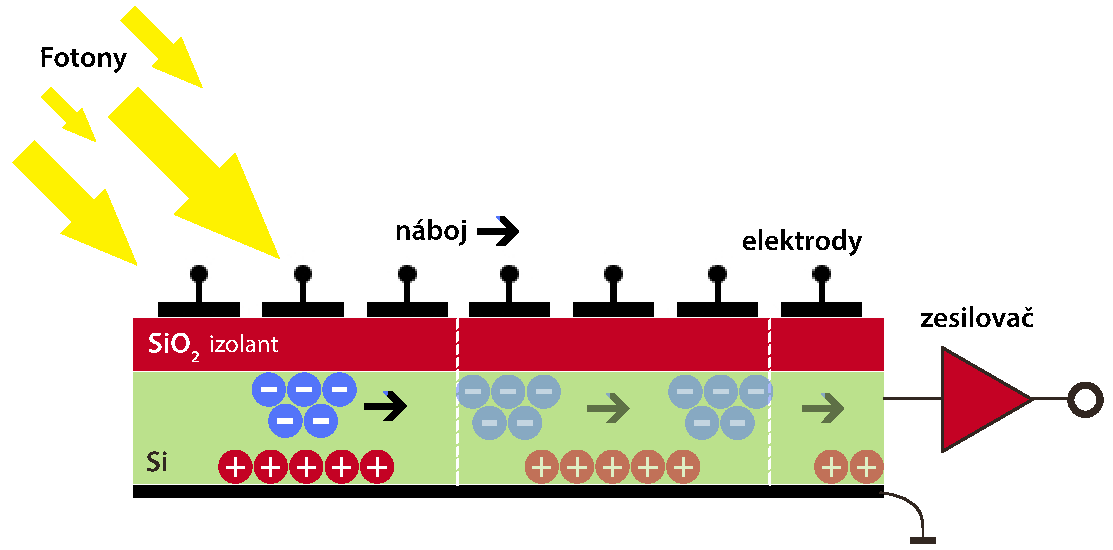
\includegraphics[width=12cm]{images/ccd.pdf}
\caption{Schéma zpracování náboje v CCD}
\label{fig:ccd}
\end{center}
\end{figure}
		
Tímto způsobem se pixel po pixelu zpracovávají jednotlivé naměřené hodnoty. Pro zjednodušení se jedná o 1D CCD senzor, který lze nalézt např. u čtečky čárových kódů. V digitální fotografii se využívá 2D senzorů. Uvažujme, že čtení probíhá po řádcích, tak potom se nejdříve posunou všechny náboje ve sloupcích o 1 pixel (obrazový bod na senzoru), tím dostaneme řádek a následně se zpracuje celý řádek. Takto se to opakuje pro všechny řádky.

\begin{figure}[ht]
\begin{center}
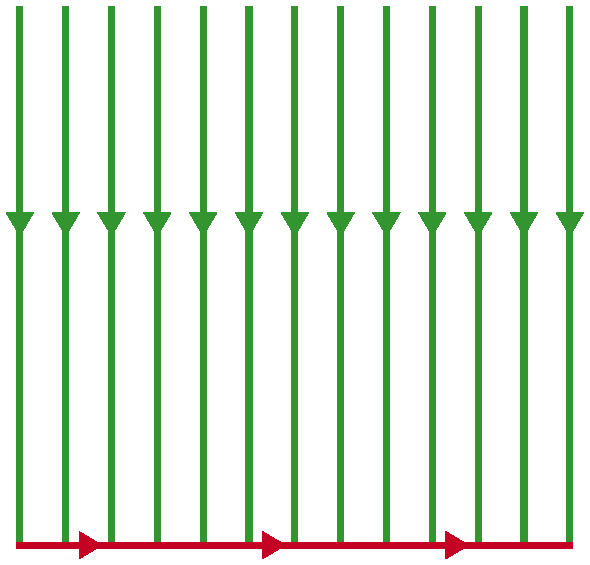
\includegraphics[width=6cm]{images/2dccd.pdf}
\caption{Znázornění zpracování CCD náboje ve 2D}
\label{fig:ccd-2d}
\end{center}
\end{figure}

V moderních fotoaparátech jsou CCD senzory spíše na ústupu. Stále se však nacházejí u modelů značek Hasseblad nebo Leica, které se spíš, než na digitální fotoaparát jako multimediální zařízení nejen pro fotografování, ale i pro natáčení videa, soustředí především na obrazový záznam. Více toto rozebereme ještě v sekci~\ref{subsec:srovnani-ccd-cmos} věnující-se srovnání s technologií CMOS.

\paragraph{Blooming}\label{subsubsec:blooming} je jev, ke kterému dochází u CCD senzorů ve chvíli, kdy na povrch snímače dopadne takové množství světla, že kapacita pixelu se naplní a elektrony se roztečou. Na obrazu tak vznikají čáry tam, kde elektrony přetekly v rámci jednoho kanálu do svého okolí. K tomu dochází především u silných světelných zdrojů, např. při fotografován proti slunci.

\begin{figure}[ht]
\begin{center}
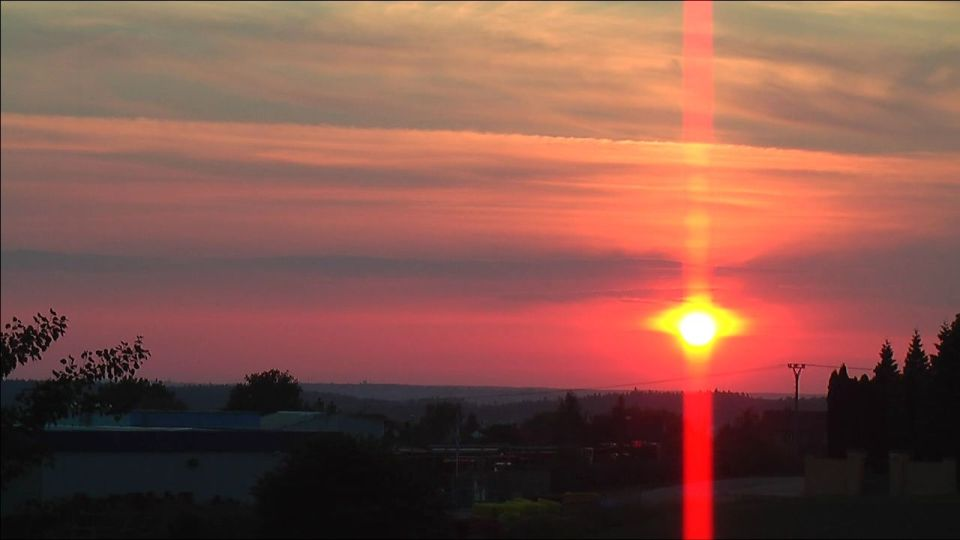
\includegraphics[width=12cm]{images/blooming.jpg}
\caption{Blooming v protisvětle v podobě červeného vertikálního pruhu}
\label{fig:blooming}
\end{center}
\end{figure}

\subsection{CMOS}\label{subsec:cmos}

Konstrukce CMOS-u a i důvod proč se jich využívá stále častěji, stojí na principu, že snímač je pole jednotlivých pixelů a každý pixel obsahuje \textbf{fotodiodu} k detekci světla, za kterou je i veškerá elektronika pro každý daný bod zvlášť (zesilovač, A/D převodník, reset/transfer gate).

\begin{figure}[ht]
\begin{center}
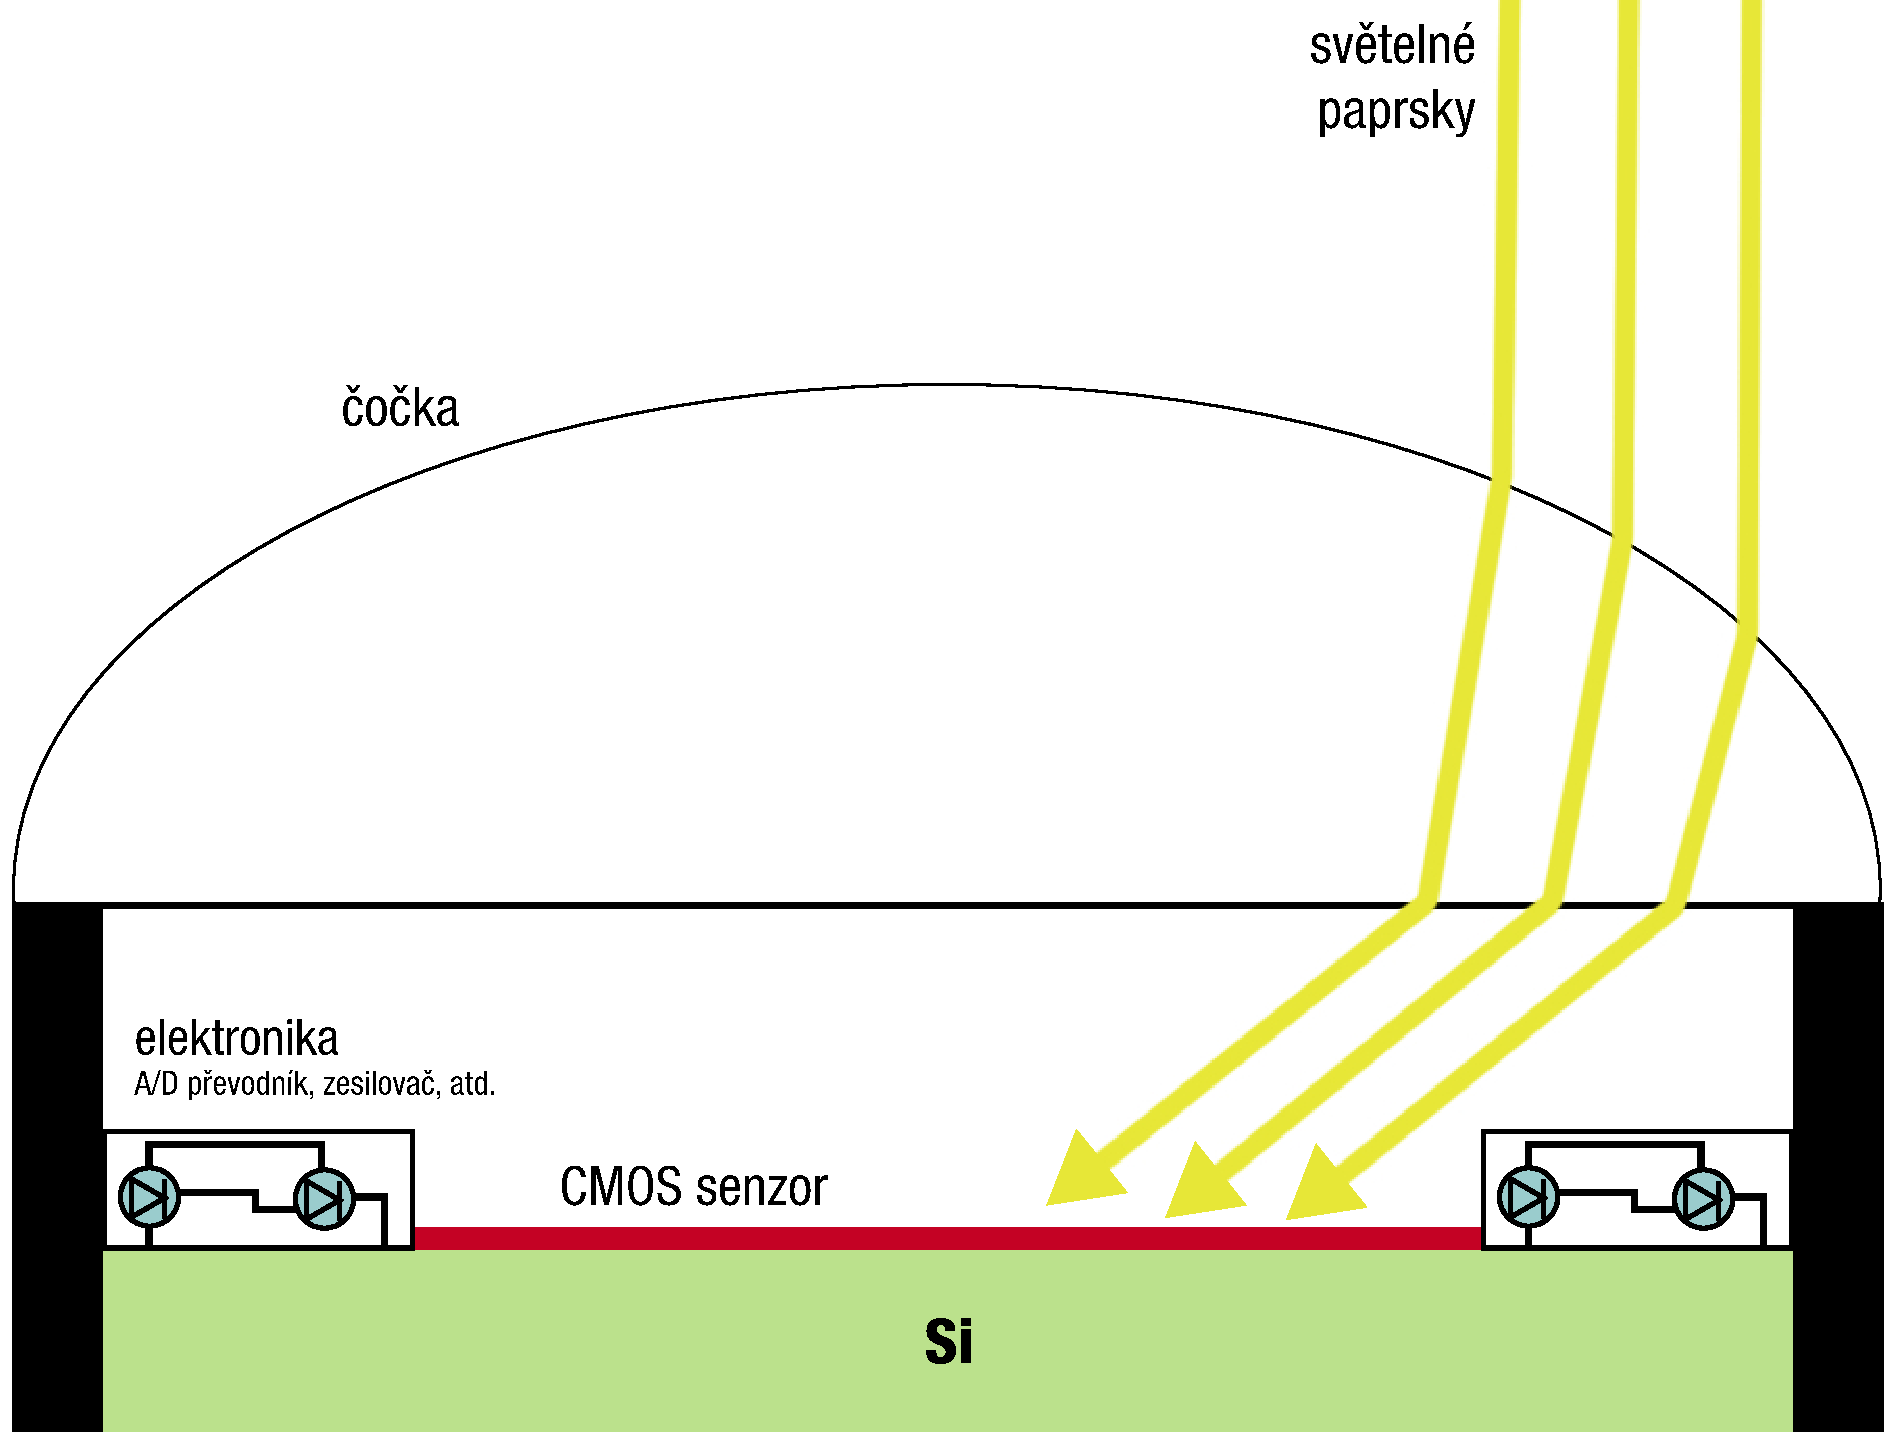
\includegraphics[width=10cm]{images/cmos-schema.pdf}
\caption{Schéma CMOS snímače}
\label{fig:cmos-schema}
\end{center}
\end{figure}

Každý pixel se tak zpracovává sám, což umožňuje přímou adresaci každého bodu již na snímači. Lze tak podstatně rychleji zpracovávat obraz i video nebo vytvářet více virtuálních obrazovek přímo ze senzoru.

\begin{figure}[ht]
\begin{center}
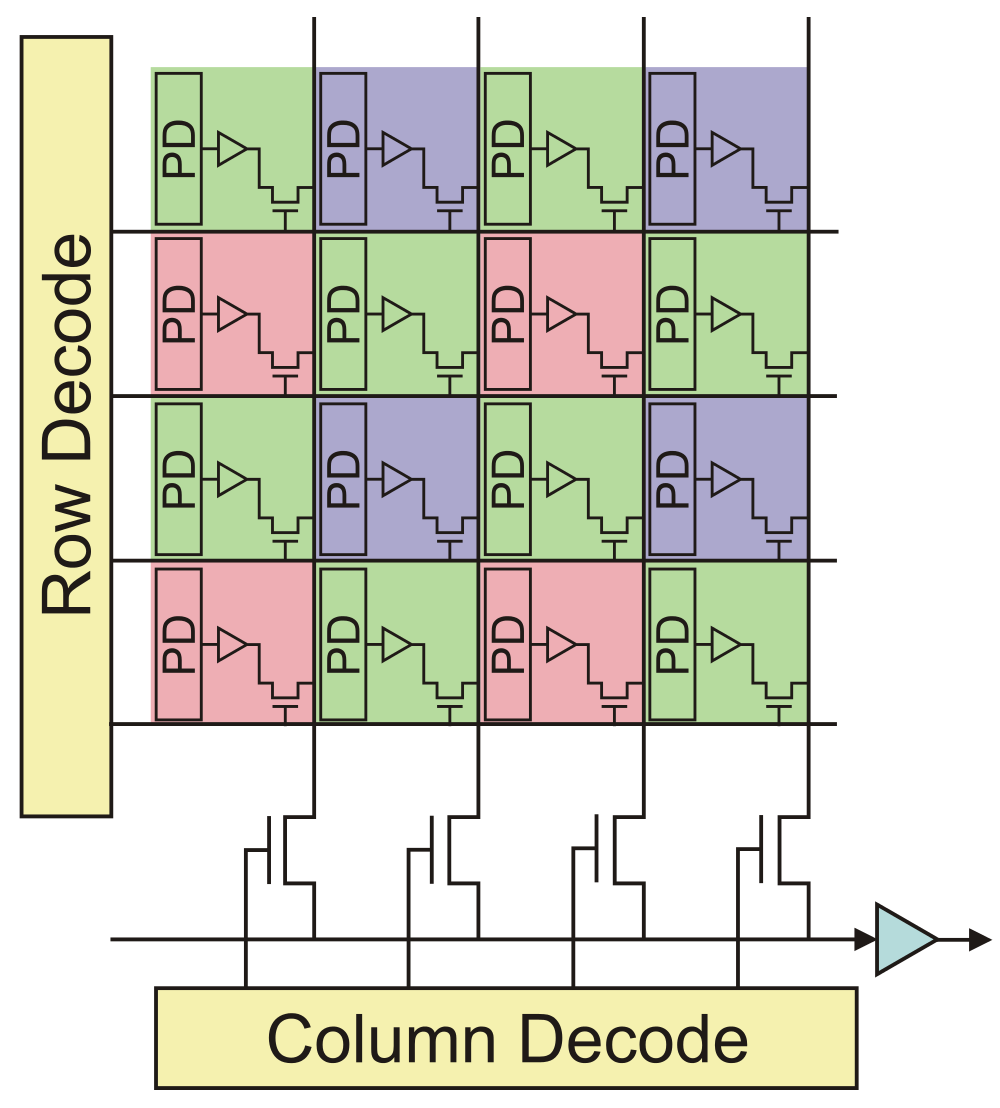
\includegraphics[width=6cm]{images/cmos-address.png}
\caption{Přímá adresace CMOS pixelů}
\label{fig:cmos-address}
\end{center}
\end{figure}

\subsubsection{BIS CMOS}\label{subsubsec:bis-cmos}

BIS\footnote{Back-Illuminated Sensor, taktéž se lze setkat se zkratkami BSI nebo BI od Backside Illumination} CMOS je technologie senzorů, která se poprvé objevila dostupná pro využití pro veřejnost kolem roku 2009 společností OmniVision Technologies, následně v jejím výzkumu dodnes pokračuje i Sony, které přineslo mnohá vylepšení. Tyto senzory lze nalézt v zařízeních jako Apple iPhone 4 nebo HTC EVO 4G.

Problém klasických CMOS-ů je ten, že většina "drátů" je na povrchu senzoru. Ty jsou sice pokryty odrazivým materiálem, takže světlo je odraženo a neruší při zpracování, ale je tak ztraceno 30\% až 40\% fotonů. To vede k problémům při fotografování ve špatných světelných podmínkách (málo světla), kdy menší množství dopadeného světla moc nepomáhá.

BIS CMOS tento problém řeší tak, že při výrobě se křemíková destička otočí a zadní strana se ztenčí, tak aby světlo prošlo až na fotodiodu. Výhodou je, že následně dochází jen k minimálním světelným ztrátám a takovéto senzory jsou vhodnější pro fotografování i za špatných světelných podmínek. Začínají se však objevovat problémy s s parazitními náboji\footnote{cross-talk} na sousedních obvodech, které se projevují jako šum nebo barevné defekty. Jejich přínos je tak především pro bezpečnostní kamery nebo právě smartphony.

\paragraph{Oči hlavonožců a obratlovců} jsou trefným příkladem tohoto principu ze zvířecí říše. Obratlovci mají nervy vytaženy na povrch sítnice, vzniká tak něco čemu říkáme slepá skvrna, na kterou když dopadá světlo, tak ho nevidí, což se dá přirovnat ke klasickému CMOS-u. Hlavonožci (sépie, chobotnice, krakatice atp.) na druhou stranu mají BIS CMOS oči - nervy jsou umístěny pod sítnicí, a tak žádnou slepou skvrnu nemají.

\subsection{Srovnání CCD a CMOS}\label{subsec:srovnani-ccd-cmos}

Využívá se stále obou technologií. CMOS senzory jsou na vzestupu především u moderních DSLR, které už neslouží nejen k fotografování, ale lze v nich fotografii upravovat nebo natáčet video. CCD jsou naopak stále využívány pro lepší obrazovou kvalitu především u profesionálních zařízení pro velkoformátovou fotografii nebo v medicíně.

\begin{itemize}
	    	\item \textbf{Výhody CMOS}				
	    	\begin{itemize}
				\item levnější na výrobu, menší spotřeba (až 100x) - nižší teploty
				\item rychlejší zpracování - přímý diskrétní výstup umožňuje rychlejší zpracování a především natáčení videa
				\item odolnost proti bloomingu - přetékání světla do okolních pixelů
	    	\end{itemize}

			\item \textbf{Výhody CCD}
			\begin{itemize}
				\item lepší obrazová kvalita (CCD může mít více bodů na stejnou plochu), protože nemá elektroniku na chipu, která by snižovala množství dopadajícího světla, technologie je citlivější na světlo
				\item lepší funkčnost za špatných světelných podmínek a méně šumu
				
			\end{itemize}
		\end{itemize}	

\paragraph{Live view} je dalším případem, který umožňují CMOS snímače. Jedná se o režim živého náhledu, který je typický pro fotoaparáty s elektronickým hledáčkem, kdy v hledáčku se zobrazují data ze snímače. U kompaktních fotoaparátu je tento režim již standardem. V roce 2007 ho představil i Canon u prvních DSLR a to Canon EOS 1Ds Mark III a Canon EOS 40D u DSLR. U CCD nedochází k natolik rychlému zpracování, aby byl výsledný obraz dostatečně plynulý. Zajímavý je i fakt, že zaostřování v tomto režimu se u DSLR provádí softwarově. Jsou porovnávaný jednotlivé snímky a procesor fotoaparátu se snaží zjistit, zda-li ten nový je ostřejší než-li ten předchozí. Takto se postupně dostane až k maximálně ostrému obrazu.


\section{Color Filter Array}\label{sec:cfa}

Sami o sobě nejsou snímače schopny určit barvu, resp. vlnovou délku dopadajícího světla. Tento problém řeší vrstva barevného filtru\footnote{angl. CFA nebo-li Color Filter Array, případně se ještě používá CFM - color filter mosaic} na vrchu snímače. Přes každý obrazový bod je barevná vrstva, která filtruje pouze světlo dané barvy (o konkrétní vlnové délce).

Výsledná barva, která je reprezentována trojicí RGB (red, green, blue), je následně vypočítána demozaikovacím algoritmem, tedy interpolací naměřených hodnot v okolí každého obrazového bodu. Tento proces se provádí buď uvnitř fotoaparátu, kde výstupem je JPEG nebo TIFF nebo pomocí specializovaného softwaru z RAW souboru.

Samotné barevné filtry se vyrábějí v různých provedeních. Nejčastější je RGGB provedení též nazývané Bayerův filtr nebo Bayerova maska po jeho vynálezci Brycei Bayerovi z Kodaku. Jedná se o čtveřice - červená, zelená, zelená, modrá. Zelená je zde dvakrát proto, že lidské oko je nejcitlivější právě na zelenou, a tak je příhodné mít nejpřesnější měření právě pro ni.

\begin{figure}[ht]
\begin{center}
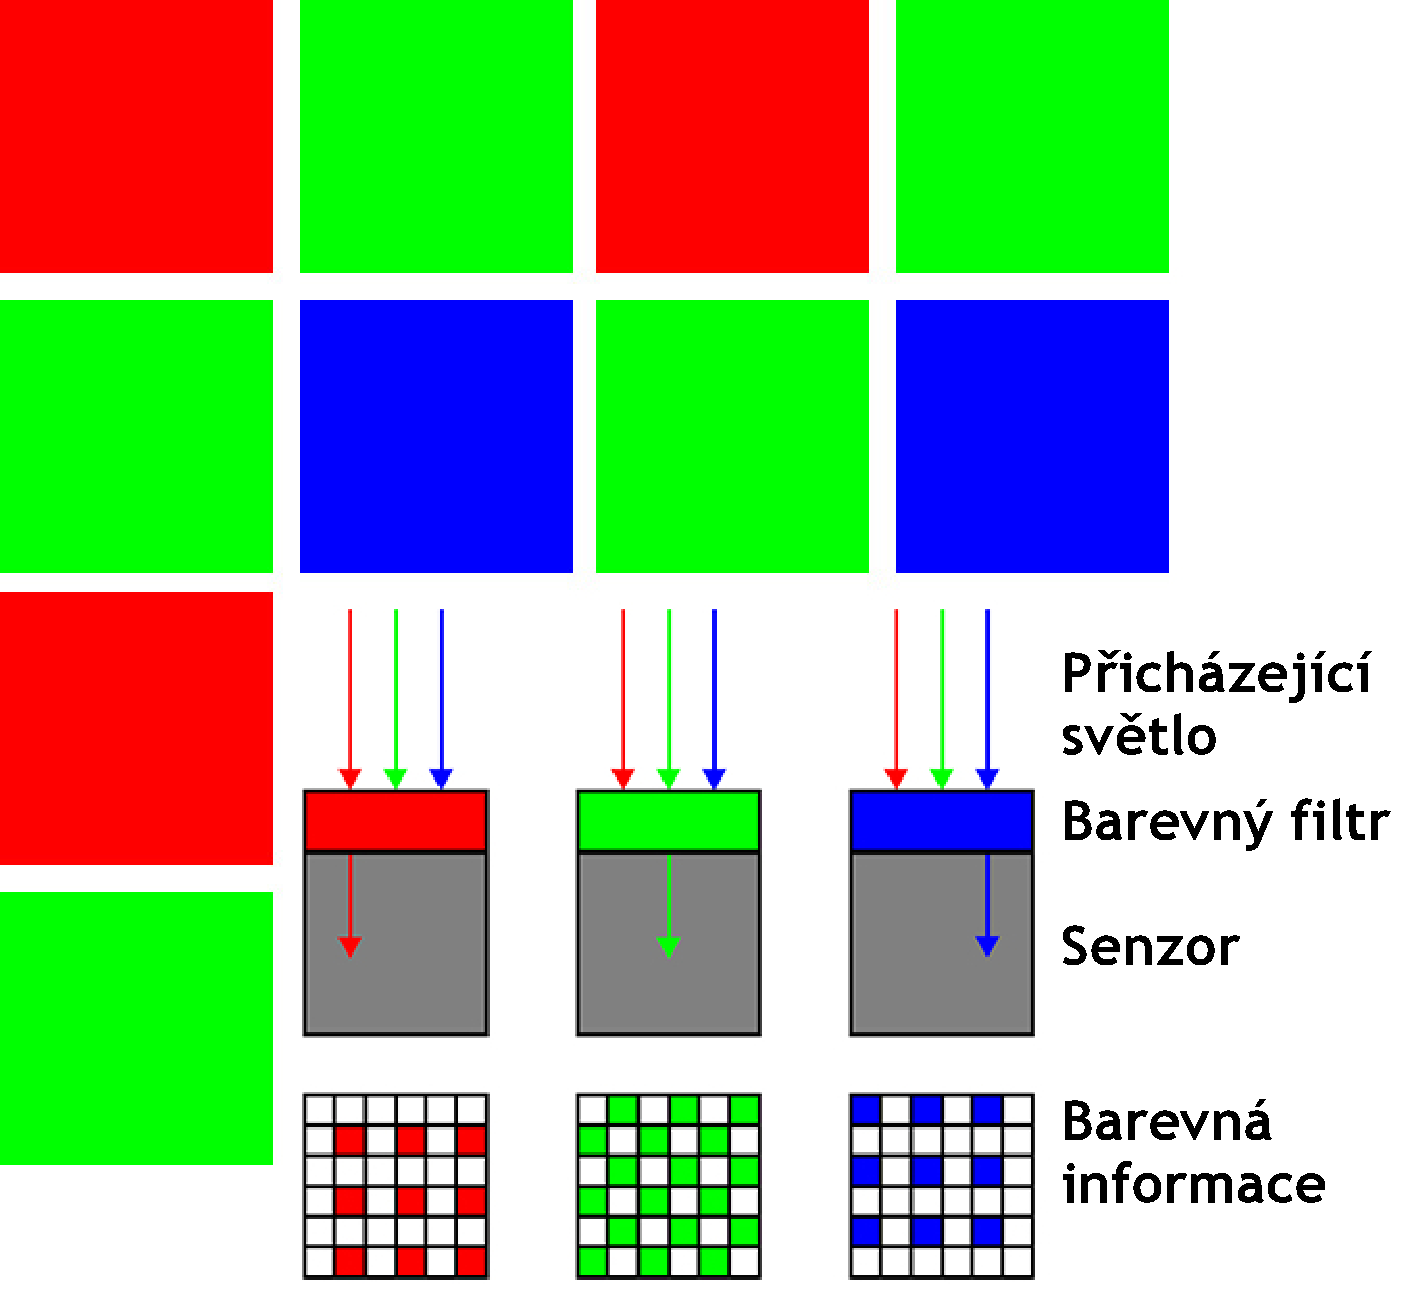
\includegraphics[width=8cm]{images/bayer-mask.pdf}
\caption{Princip fungování Bayerova filtru}
\label{fig:bayer}
\end{center}
\end{figure}

Další provedení barevných senzorů jsou (C (cyan) - azurová, Y (yellow) - žlutá, M (magenta) - purpurová, W (white) - bílá), E (emerald - varianta zelené):
\begin{itemize}
	\item RGBE 
	\item CYYM
	\item CYGM
	\item RGBW
\end{itemize}

Jiných barevných provedení, než-li RGB, se využívá opět za účelem naměření více světla. Výsledná barva se pak počítá zcela odlišným způsobem.

\paragraph{Foveon X3} je speciálním případem snímače, který používá odlišný princip zjištění barvy od klasických CFA. Nejedná se ani tak o barevnou mozaiku, ale o 3 barevné vrstvy nad sebou - červenou, zelenou, modrou, kde nejdříve se naměří celková hodnota, následně se odfiltruje modrá složka, zelená a nakonec červená složka. Rozdílově tak zjistíme kompletní barevnou informaci pro každý obrazový bod a není tak třeba demozaikovacího algoritmu k výpočtu barvy. Dnes tuto technologii používají fotoaparáty značky Sigma. 

\begin{figure}[ht]
\begin{center}
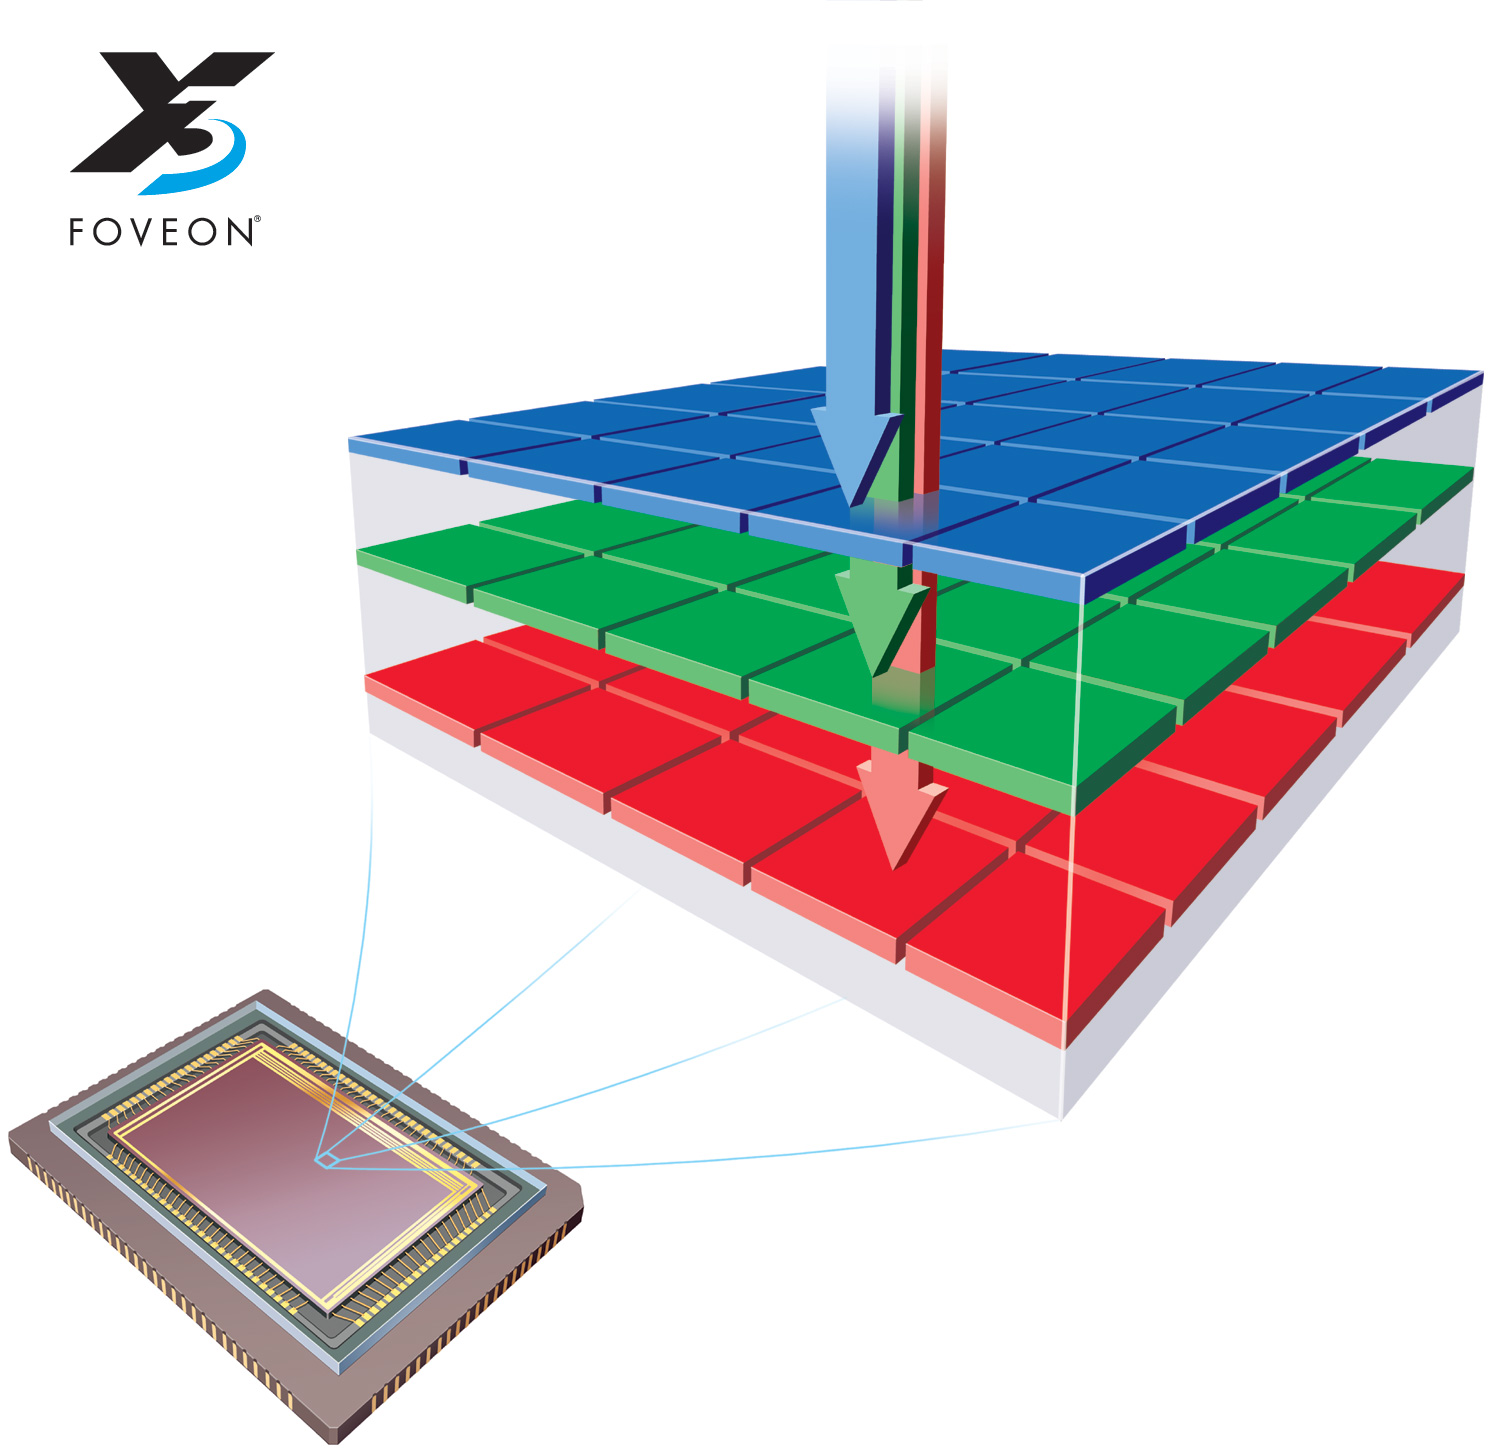
\includegraphics[width=8cm]{images/foveon-cfa.jpg}
\caption{Foveon X3 sensor}
\label{fig:foveon}
\end{center}
\end{figure}

\chapter{RAW}

RAW není zkratka, ale značí se tak surový výstup z fotoaparátu. K RAW se pojí i další pojmy jako digitální temná komora\footnote{jedná se o analogii procesu vyvolávání fotografie v temné komoře, avšak digitálně} nebo digitální negativ\footnote{Při negativním procesu vyvolávání fotografie se nejdříve vyvolá negativ a následně ten se přes zvětšovák nasvítí na fotografický papír, který se pak opět vyvolá. Taktéž DNG (Digital Negative) je zkratka RAW formátu od Adobe.}. To proto, že tento výstup nedává sám o sobě obraz, ale slouží pouze k jeho vytvoření.

\begin{figure}[ht]
\begin{center}
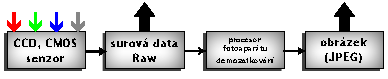
\includegraphics[width=14cm]{images/chain.pdf}
\caption{Postup zpracování obrazu uvnitř digitálního fotoaparátu}
\label{fig:chain}
\end{center}
\end{figure}

U hlavních výrobců digitálních fotoaparátů se můžeme setkat s těmito formáty:

\begin{itemize}
	\item \verb|DNG| (Adobe, Pentax)
	\item \verb|CR2| (Canon)
	\item \verb|NEF| (Nikon)
	\item \verb|ORF| (Olympus)
	\item \verb|ARW| (Sony)
\end{itemize} 

V září roku 2004 se pokusila společnost Adobe formát \verb|DNG| standardizovat, nicméně jejich snaha se nesetkala s úspěchem a jediný kdo \verb|DNG| převzal byl Pentax. Vznikl tak další formát, který má tu výhodu, že je založen na obecné specifikaci TIFF/EP\footnote{standard pro digitální obrazové formáty - ISO 12234-2, nejedná se o to samé jako formát TIFF, ale pouze jeho rozšíření, společně s rozšířením pro EXIF - specifikací tagů užívaných u zvukových a obrazových formátů, více se lze dočíst ve \hyperlink{bib}{specifikaci}}, má veřejně dostupnou dokumentaci, specifikaci a SDK (vývojové rozhraní).

Samotný formát je částečně specifický pro každý fotoaparát. Obsahuje surová obrazová data z daného fotoaparátu. Není však jasné o kolika bitovou informaci se jedná nebo čeho to jsou vlastně hodnoty. Tyto hodnoty se následně musí ještě zpracovat ať už procesorem fotoaparátu nebo uživatelem pomocí specializovaného softwaru.

\section{Struktura DNG}

\verb|DNG| je formát založený na specifikaci TIFF/EP, proto z hlediska kompatibility je možné \verb|DNG| soubory číst jako by se jednalo o TIFF a zpracovat tak do obrazových formátů jako \verb|JPEG| nebo \verb|TIFF|.

\subsection{EXIF, TIFF/EP, IPTC, XMP a metadata}

Kromě samotné barevné informace obsahuje \verb|DNG| ještě velké množství dalších informací - metadat. Nejen o čase, clonovém čísle, ISO nebo např. GPS souřadnic. Tedy za jakých okolností byla fotografie pořízena, ale i informací potřebných pro zpracování obrazových dat.

K ukládání metadat používá \verb|DNG| tagy \verb|TIFF/EP|, \verb|EXIF|, \verb|IPTC| a \verb|XMP| a to v \verb|SubIFD|\footnote{sub-Image File Directory - systém složek pro obrazové formáty} stromech dle specifikace \verb|TIFF/EP|. V praxi se nejedná o nic jiného, než-li o stromovou strukturu, ve které se nacházejí tagy jednotlivých metadat a jejich obsah. Případné proprietární informace výrobců, kteří chtějí \verb|DNG| využívat se nacházejí ve speciálních \verb|DNG| tagích pod položkou DNGPrivateData.

\paragraph{EXIF}\footnote{Exchangeable image file format} je soubor metadat používaných pro zvuk a obraz používaný např. ve formátech \verb|TIFF|, \verb|JPEG|, \verb|WAV|. Specifikace se dělí na část zvukovou (Exif audio file specification) a část obrazovou (Exif image file specification). Kromě informací o datu a čase, nastavení fotoaparátu a copyrightu, obsahuje i náhled obrazu používány při prohlížení na displayi fotoaparátu nebo v softwaru.

\paragraph{IPTC}\footnote{International Press Telecommunications Council} je podstatně obecnejší standard pro metadata všech možné typů. Z části se překrývá s \verb|EXIF|-em.

\paragraph{XMP}\footnote{Extensible Metadata Platform} je ISO standard vytvořený společností Adobe ke zpracování všech možných typů metadat. Jedná se tak o datový model ve formátu \verb|XML|.

\subsection{Profil fotoaparátu}\label{subsec:profil-fotoaparatu}

Profil fotoaparátu je dán následujícími obsahem následujících \verb|DNG| tagů:

\begin{itemize}
	\item ColorMatrix1
	\item ColorMatrix2
	\item ReductionMatrix1
	\item ReductionMatrix2
	\item CalibrationIlluminant1
	\item CalibrationIlluminant2
	\item ProfileCalibrationSignature
	\item ProfileName
	\item ProfileHueSatMapDims
	\item ProfileHueSatMapData1
	\item ProfileHueSatMapData2
	\item ProfileToneCurve
	\item ProfileEmbedPolicy
	\item ProfileCopyright
	\item ForwardMatrix1
	\item ForwardMatrix1
	\item ProfileLookTableDims
	\item ProfileLookTableData
\end{itemize}

Těchto dat se využívá pří zpracování do podoby obrazu o čemž se více dozvíte v sekci \ref{sec:zpracovani-raw}. Bez nich by nebylo možné zkonstruovat výsledný obraz. Pozor, tyto tagy určují pouze profil fotoaparátu, nejedná se o všechny \verb|DNG| tagy potřebné k vyvolání obrazu.

\subsection{Opcode Lists}

Opcode Lists jsou další zajímavou informací. Dělí se do 3 strukturálních částí, kde v první jsou informace uloženy ve 32-bitových celých číslech\footnote{32-bit unsigned integer} a v dalších dvou v hodnotách od 0.0 do 1.0. Těchto dat se využívá při zpracování obrazu k operacím jako warping\footnote{transformace obrazu jako soudkovitost nebo perspektiva, využívá se i pro odstranění chromatické aberace}, vinětace, zvětšování, zmenšování nebo odstranění vadných pixelů.

\section{Zpracování RAW}\label{sec:zpracovani-raw}

Ve chvíli kdy dostaneme do ruky obrazová data z RAW, jedná se o nezpracovaná data, kde není zřejmé, o co se jedná - jaká je bitová hloubka této informace? V jakém rozsahu jsou tyto čísla? Jedná se o trojice čísel nebo o jednorozměrnou informaci? Popř. jaký je použit barevný filtr, abychom věděli jaká hodnota odpovídá které barvě? Při zpracování se musí projít následujícími kroky a využívá se \verb|DNG| tagů..

\paragraph{1. Oříznutí a určení bílé a černé úrovně} RAW data obsahují černý rámeček, který určuje černou úroveň, která je uvedena i v tagu BlackLevel. Dále je potřeba ještě tagů WhiteLevel a  Tato úroveň je uvedena i v tagu BlackLevel, ActiveArea a DefaultCropSize. Od všech hodnot se zde odečte BlackLevel a vydělí rozdílem BlackLevel a WhiteLevel. Tím dostaneme hodnoty mezi 0.0 a 1.0, které se následně zpracovávají. Rámeček pak již není potřeba a pomocí ActiveArea a DefaultCropSize se ořízne.

\begin{figure}[ht]
\begin{center}
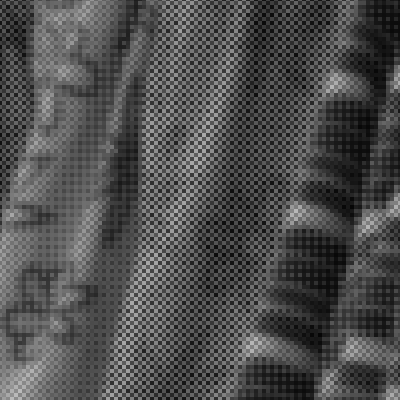
\includegraphics[width=6cm]{images/e_nonwb.png}
\caption{Zpracovaná černá a bílá úroveň}
\label{fig:non-wb}
\end{center}
\end{figure}

\paragraph{2. Vyvážení bílé} je proces, kdy se nastavuje barevná teplota\footnote{Barevná teplota, nebo-li chromatičnost, charakterizuje spektrum bílého světla. Způsobuje zabarvení od červené, je-li nastavena vyšší barevná teplota, do modré, je-li nastavena nižší. Lidské oko toto řeší pamětí barev, kdy si mozek pamatuje jakou má co barvu, a tak se přizpůsobuje.} výslednému obrazu. Koeficienty vyvážení bílé jsou uvedeny v AsShotNeutral, a to pro každou barvu barevného filtru, je tak třeba znalost jeho uspořádání (RGGB, RGBG, CYYM, atd.).

\begin{figure}[ht]
\begin{center}
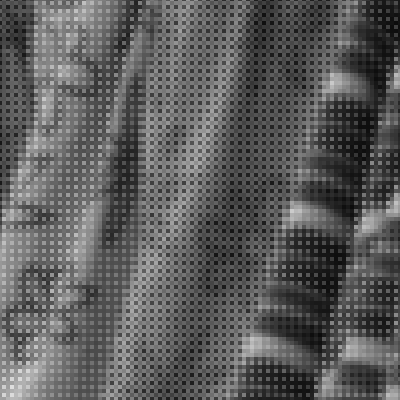
\includegraphics[width=6cm]{images/e_wb.png}
\caption{Po vyvážení bílé}
\label{fig:white-balanced}
\end{center}
\end{figure}

\paragraph{3. Demozaikování} viz. \ref{subsec:demozaikovani}

\begin{figure}[ht]
\begin{center}
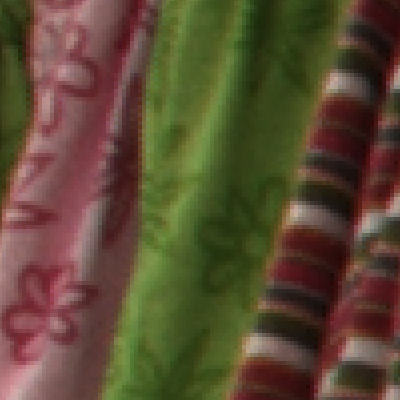
\includegraphics[width=6cm]{images/e_demosaiced.png}
\caption{Demozaikovaná fotografie obsahující barevnou informaci}
\label{fig:demosaiced}
\end{center}
\end{figure}

\paragraph{4. Určení barevného profilu} V tuto chvíli již existuje koukatelný barevný obraz. Pokud bychom chtěli takovýto obraz zobrazit na monitoru, byly by jeho barvy mdlé. Jedná se o barvy v barevném prostoru fotoaparátu, který je schopný zachytit více barev, než zobrazuje monitor. Např. jeho nejsytější zelené už nejsou na monitoru zobrazitelné. Navíc monitor neví kolik barev je fotoaparát schopen zachytit, což se liší model od modelu. Je tedy třeba převést tyto barvy do barevného prostoru, který je všeobecně znám. K tomu slouží údaj ColorMatrix, který obsahuje matici přepočtu z CIE XYZ\footnote{CIE XYZ je univerzální barevný prostor, který krom vědeckých účelů, slouží i jako nadmnožina ostatních barevných prostorů. Je tak využíván pro jejich vzájemné převody.} do barevného prostoru fotoaparátu. Pomocí této matice se převedou hodnoty do CIE XYZ, z čehož už lze převést hodnoty dále na standardně používané profily jako sRGB\footnote{sRGB je standard používaný všude. Není-li známo jaký barevný profil se používá, automaticky se uvažuje právě sRGB.} nebo Adobe RGB\footnote{Adobe RGB je barevný profil obsahující širší gamut, než-li sRGB. Je tak využíván především fotografy nebo grafiky, kdy výsledným médiem je kvalitní monitor nebo tisk.}, se kterými si poradí většina zobrazovacích zařízení.

\paragraph{5. Postprocessing}

V tuto chvíli je fotografie zpracována. Hodnoty od 0.0 do 1.0 lze převést na 8-bitový nebo 16-bitový barevný rozsah, provádět úpravy jako změna kontrastu, jasu nebo sytosti, které už jsou čistě subjektivní a uložit do některého z obrazových formátů.

\subsection{Demozaikování a interpolace barev} \label{subsec:demozaikovani}

Demozaikování je proces, který z hodnot naměřených pomocí barevného filtru (viz. \ref{sec:cfa}) vytvoří barevný obraz, kde každému pixelu odpovídá přesně daná barva (RGB, CMYK, atd.). Je třeba znát konstrukci CFA a následně pomocí interpolace hodnot (průměrování) v okolí každého pixelu se vypočítá jeho hodnota.

\begin{figure}[ht]
\begin{center}
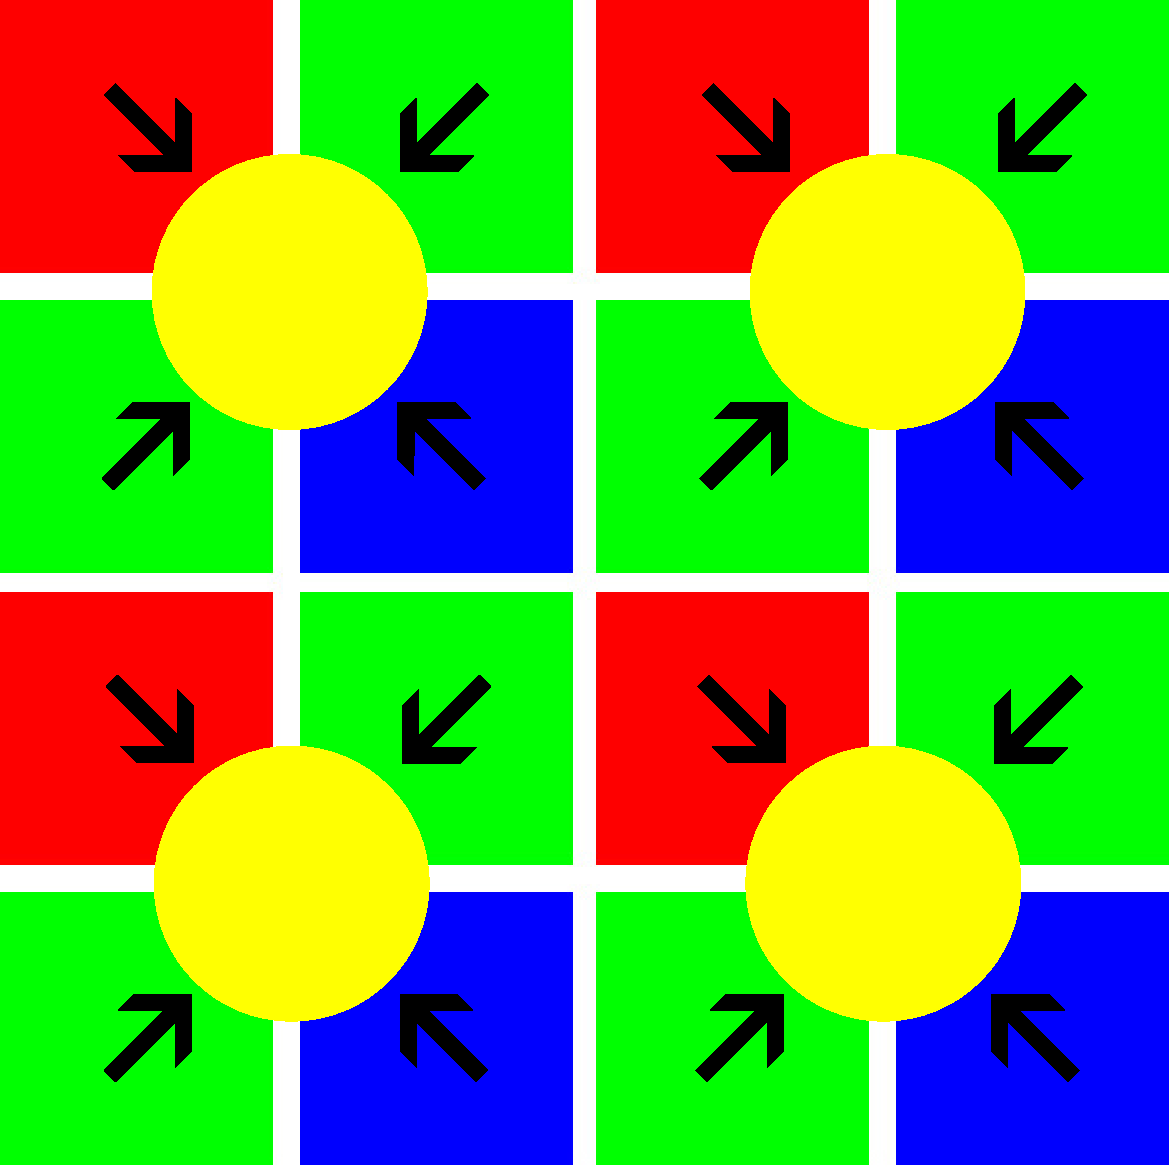
\includegraphics[width=6cm]{images/bayer-interpolation.pdf}
\caption{Interpolace barev z Bayerova filtru}
\label{fig:bayer-inter}
\end{center}
\end{figure}

K interpolaci se používají různé algoritmy, které produkují odlišné výsledky. V softwaru si lze tento algoritmus často zvolit, ve fotoaparátu tomu tak není. Mezi používané algoritmy patří interpolace dle nejbližšího souseda, bilineární interpolace, bikubická, Lancoszova.

\subsection{RAW konvertory}

Obraz z RAW dokáže zpracovat nejen digitální fotoaparát, ale i specializovaný software - RAW konvertor. Výstup z fotoaparátu je tradičně ukládán jako \verb|JPEG| na paměťovou kartu. Software vhodný pro zpracování RAW čítá:

\begin{itemize}
	\item Adobe Lightroom, Adobe Camera Raw (plug-in)
	\item Zoner Photo Studio
	\item RawTherapee
	\item Software jednotlivých výrobců (Nikon Capture NX, Canon Digital Photo Professional)
\end{itemize}

Nevýhodou softwaru třetí strany, kterým jsou např. produkty od Adobe nebo Zoneru, je že dodané RAW často není ve formátu \verb|DNG|, ale ve formátu daného výrobce, kde je zpracování specifické pro každý fotoaparát. Musí se tak čekat, než-li autor softwaru přidá podporu pro daný model.

\subsection{Výhody a nevýhody zpracování z RAW}

\paragraph{Výhody}
	    		\begin{itemize}
	    			\item zpracování v 12/14-bit barevné hloubce (podle výrobce senzoru) - umožňuje širší dynamický rozsah, než-li 8-bit JPEG
	    			\item vlastní nastavení doostření, barevné teploty, jasu, kontrastu
	    			\item nedestruktivní úprava - informace o úpravách se ukládají buď do externího XMP souboru nebo přímo do hlavičky RAW
	    		\end{itemize}	



\paragraph{Nevýhody}
	    		\begin{itemize}
	    			\item velké soubory (výjimka 16-bit TIFF, který je větší)
	    			\item časová náročnost zpracování
	    			\item kompatibilita RAW konvertorů a novějších fotoaparátů (DNG Convertor)
	    		\end{itemize}


%---------------------------------------------------------------------------

\bibliographystyle{plain}

\nocite{cite1}
\nocite{cite2}
\nocite{cite3}
\nocite{cite4}
\nocite{cite5}
\nocite{wiki1}
\nocite{wiki2}
\nocite{wiki3}

\hypertarget{bib}{}
\bibliography{reference}
\addcontentsline{toc}{chapter}{Literatura}

\appendix

\chapter{Seznam použitých zkratek}

\begin{description}
\item[APS-C] Advanced Photo System type-C
\item[BIS] Back-illuminated sensor
\item[BI] Backside illumination
\item[CCD] Charge-coupled device
\item[CFA] Color Filter Array
\item[CFM] Color Filter Mosaic
\item[CMOS] Complementary metal–oxide–semiconductor
\item[CMYK] Cyan Magenta Yellow Black
\item[DSLR] Digital single-lens reflex camera
\item[EXIF] Exchangeable Image File Format
\item[IFD] Image File Directory
\item[IPTC] International Press Telecommunications Council
\item[JPEG] Joint Photographic Experts Group
\item[RGB] Red Green Blue
\item[TIFF] Tag Image File Format
\item[TIFF/EP] Tag Image File Format / Electronic Photography
\item[XMP] Extensible Metadata Platform
\end{description}
\vdots

\chapter{Instalační a uživatelská příručka}

K dokumentu jsou přiloženy soubory \verb|raw.m| a \verb|raw.fig|. \verb|raw.fig| obsahuje GUI, tudíž lze ignorovat. \verb|raw.m| je spustitelný MATLAB soubor, který je odzkoušen na MATLAB 2012a, není tak zaručena funkčnost na předchozích verzích. 

Práce s programem je celkem intuitivní. Načte se \verb|DNG| soubor a lze si proklikat jednotlivé kroky zpracování RAW, přičemž vpravo se objevuje jak v daný okamžik obraz vypadá. Obraz lze pro důkladnější prostudování uložit do \verb|JPEG|-u

Po dokončení zpracování se aktivují i posuvníky a tlačítka pro zpracování samotného obrazu, na kterých lze demonstrovat jednoduchý grafický editor.

Zpracovávat lze pouze soubory \verb|DNG|, které byly předzpracovány z libovolného RAW formátu pomocí Adobe DNG Convertoru (\href{https://www.adobe.com/support/downloads/product.jsp?product=106&platform=Windows}{ke stáhnutí zde}):

\begin{enumerate}
	\item Pod položkou 4 - Předvolby zvolte "Změnit předvolby..."
	\item Kompatibilita: Vlastní
	\item Starší verze: DNG 1.3, obě zaškrtávací políčka (Lineární (bez mozaiky), Nekomprimovaný) nezaškrtlá
	\item OK - OK - Převést
\end{enumerate}

\end{document}

